% Este arquivo .tex será incluído no arquivo .tex principal. Não é preciso
% declarar nenhum cabeçalho

\section{Jornal da Unicamp}

O jornal da Unicamp é um jornal de distribuição semanal distribuído dentro da
Unicamp. Podem-se encontrar diversos exemplares do jornal na sala de computadores
que fica ao lado da DAC, no IC-2 e em diversos pontos espalhado pelo campus.

No jornal são mostradas as diversas pesquisas realizadas pela universidade,
eventos, livros e obras de autoria de professores, aparições da Unicamp na
imprensa e defesas de mestrado e doutorado.

Na página do jornal (\url{www.unicamp.br/ju}) podem-se encontrar as
últimas edições do jornal (em PDF), além de poder fazer a assinatura online do
jornal, distribuído em formato PDF. A assinatura e distribuição do jornal são
gratuitas.

\section{Eventos da Unicamp}
\subsection{Feira do Livro}

Evento iniciado em 2002, a cada dois anos a Editora da Unicamp realiza a Feira
do Livro, no Ginásio da Unicamp. Há excelentes opções, de diversas editoras,
principalmente na área de literatura, artes e humanas, com no mínimo 50\% de
desconto.

\subsection{Semanas da Unicamp}

Alguns cursos da Unicamp realizam anualmente um evento (chamado de Semana) em
que os alunos de graduação têm um contato com o mercado de trabalho, com as
pesquisas, com as tendências e novidades dos cursos e demais assuntos, ramos
e áreas de cada curso. Para isso, participam desse evento ex-alunos
e profissionais, realizam-se palestras e minicursos, são feitas visitas
a empresas e são feitos debates ("mesas redondas").

\subsubsection{Secomp}

A computação tem a sua semana. Organizada por três entidades estudantis da computação
-- CACo, AAACEC e Conpec -- e tendo como missão “Capacitar os estudantes de computação, aproximá-los do mercado e difundir inovações em 
Tecnologia da Informação”, a Secomp -- Semana da Computação pretende mostrar ao aluno 
todas as oportunidades que existem  após a formatura, dando uma visão geral sobre o 
assunto e mostrando de perto como funcionam as possíveis carreiras.
\begin{figure}[h!]
    \vspace{-10pt}
    \centering
    
\includegraphics[scale=0.68, keepaspectratio=true]{img/imgs/secomp.jpg}
    \vspace{-10pt}
\end{figure}

Os  congressistas podem participar de palestras, treinamentos, cursos, visitas às
empresas e atividades de integração, proporcionando ao participante uma visão completa 
do mercado de TI, conforme a proposta do evento.

Se você acha que nada disso importa, bixo, você é burro, mas não tem problema. A Secomp também tem
coffee breaks até você não aguentar mais, além de uns par de brindes e prêmios
sorteados, tudo isso pelo preço de uma balada no Campinas Hall. Não perca!

\subsection{Talento}

Talento é um evento que acontece todo ano, desde 1999, durante um dia inteiro,
no Ginásio Multidisciplinar e organizado pelo Núcleo de Empresas Juniores da
Unicamp. Trata-se de uma feira de recrutamento, onde alunos da Unicamp e de
outras universidades e o público em geral têm contato com empresas, seja por
meio de palestras, mesas redondas e estandes, e estas apresentam o seu processo
seletivo. Nesse evento também é feito o cadastro de currículos dos visitantes.

Para saber mais sobre o evento, é só acessar a página da Talento
(\url{www.talentounicamp.com.br}). O evento é gratuito.

\subsection{UPA -- Unicamp de Portas Abertas}

Desde 2003 acontece a UPA (Unicamp de Portas Abertas).
\begin{figure}[h!]
    \centering
    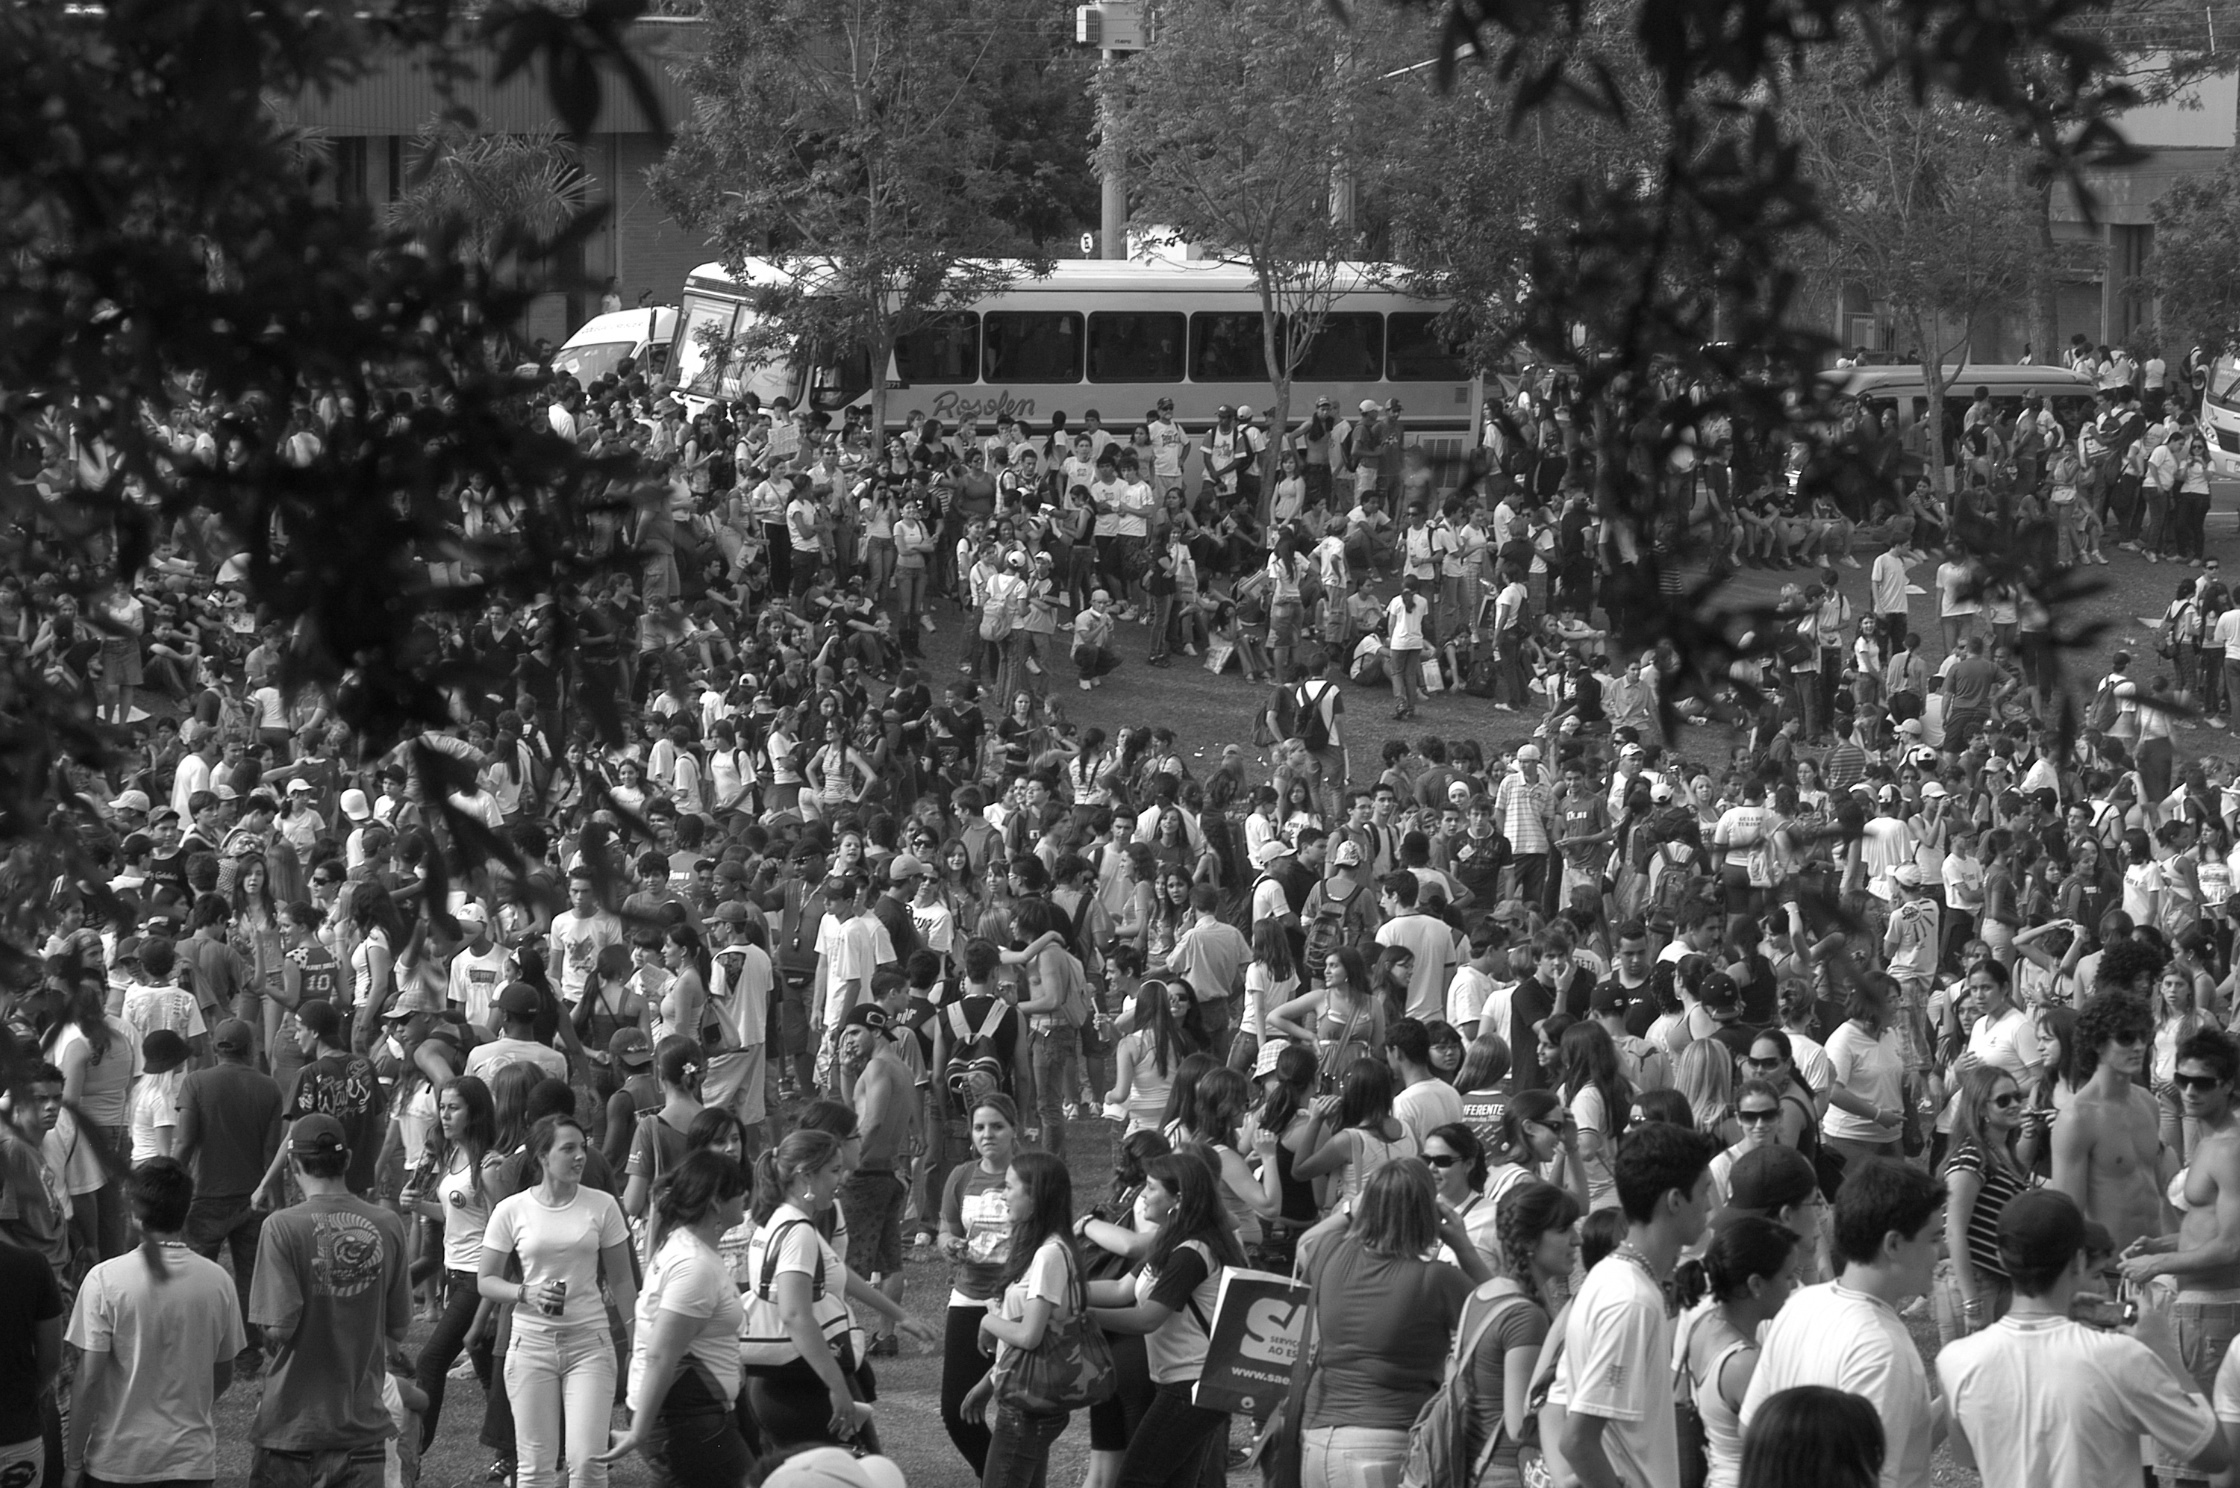
\includegraphics[scale=0.38, keepaspectratio=true]{img/imgs/bateria.jpg}
\end{figure}
Esse evento é um
aprimoramento de um evento que acontecia há alguns anos atrás, a Universidade
Aberta ao Público.

A UPA é um evento anual, em que, durantes dois dias (geralmente dois dias do mês
de setembro) a Unicamp é apresentada para estudantes dos ensinos fundamental
e médio de todo o país (muitos desses alunos sendo pré-vestibulandos). A apresentação
da universidade é feita por professores e alunos, que mostram as salas de aula
e as pesquisas realizadas.

No ano de 2011, a UPA recebeu a visita de 45 mil alunos de 670 escolas públicas
e privadas de 12 estados.

Para saber mais sobre o evento, é só acessar a página
\url{www.upa.unicamp.br}.

\section{Para que eu estou estudando isso?}

O ensino médio acabou, você finalmente está livre de todas as inutilidades, como
química orgânica e separação silábica de verbos parnasianos, só vai ver coisas
relevantes para a profissão, e{\dots}

Pimba! HZ291. Pode, Arnaldo?

Primeiro, você precisa saber que a Universidade não é um curso técnico. A ideia
não é só te dar capacitação profissional, mas sim formar pessoas melhores. Para
que um computeiro precisa de contabilidade? Para nada, mas uma pessoa (de exatas
pelo menos) precisa ter uma noção disso.

Outro problema: o que exatamente é "relevante para a sua profissão"?
A computação é uma área muito vasta, e a graduação (o curso que você tá
fazendo{\dots}) é bem generalista, para te dar base para escolher. Por exemplo,
vai ter gente que nunca mais vai usar GA/Algelin, mas quem for para a área de
computação gráfica vai comer matriz no café da manhã. Quem garante que no meio
do curso você não decida ir para essa área? Ou ainda, que no seu emprego não te
joguem um problema desse tipo?

Se você continuar na Universidade, na pós você só terá matérias da sua área, já
que você já sabe o suficiente pra dizer que área é essa. Mas ainda falta muito
chão até lá{\dots}

Para quem é da Engenharia, um problema maior é que, para conseguir o CREA,
existem algumas matérias obrigatórias (embora completamente inúteis, sem
exagero), como Resistência dos Materiais. A Unicamp pode até contrariar essas orientações, até
certo ponto, mas dificilmente os professores concordariam. (Por outro lado,
você poderá construir prédios de até 2 andares. Recomendamos fortemente que você
não faça isso.)

Para quem é da Ciência, o curso não é para formar "programadores". Vocês serão
mais que isso, serão cientistas, e isso envolve ver coisas além de só código.
